\section{Datenaufbereiterung und Speicherung}
In diesem Abschnitt betrachten wir den Teil der Datenpipeline, in dem die Daten heruntergeladen und anschließend im \emph{Skript 1} aufbereitet und gespeichert werden.

\begin{figure}[h!]
    \vspace{0.7cm}
    \centering
    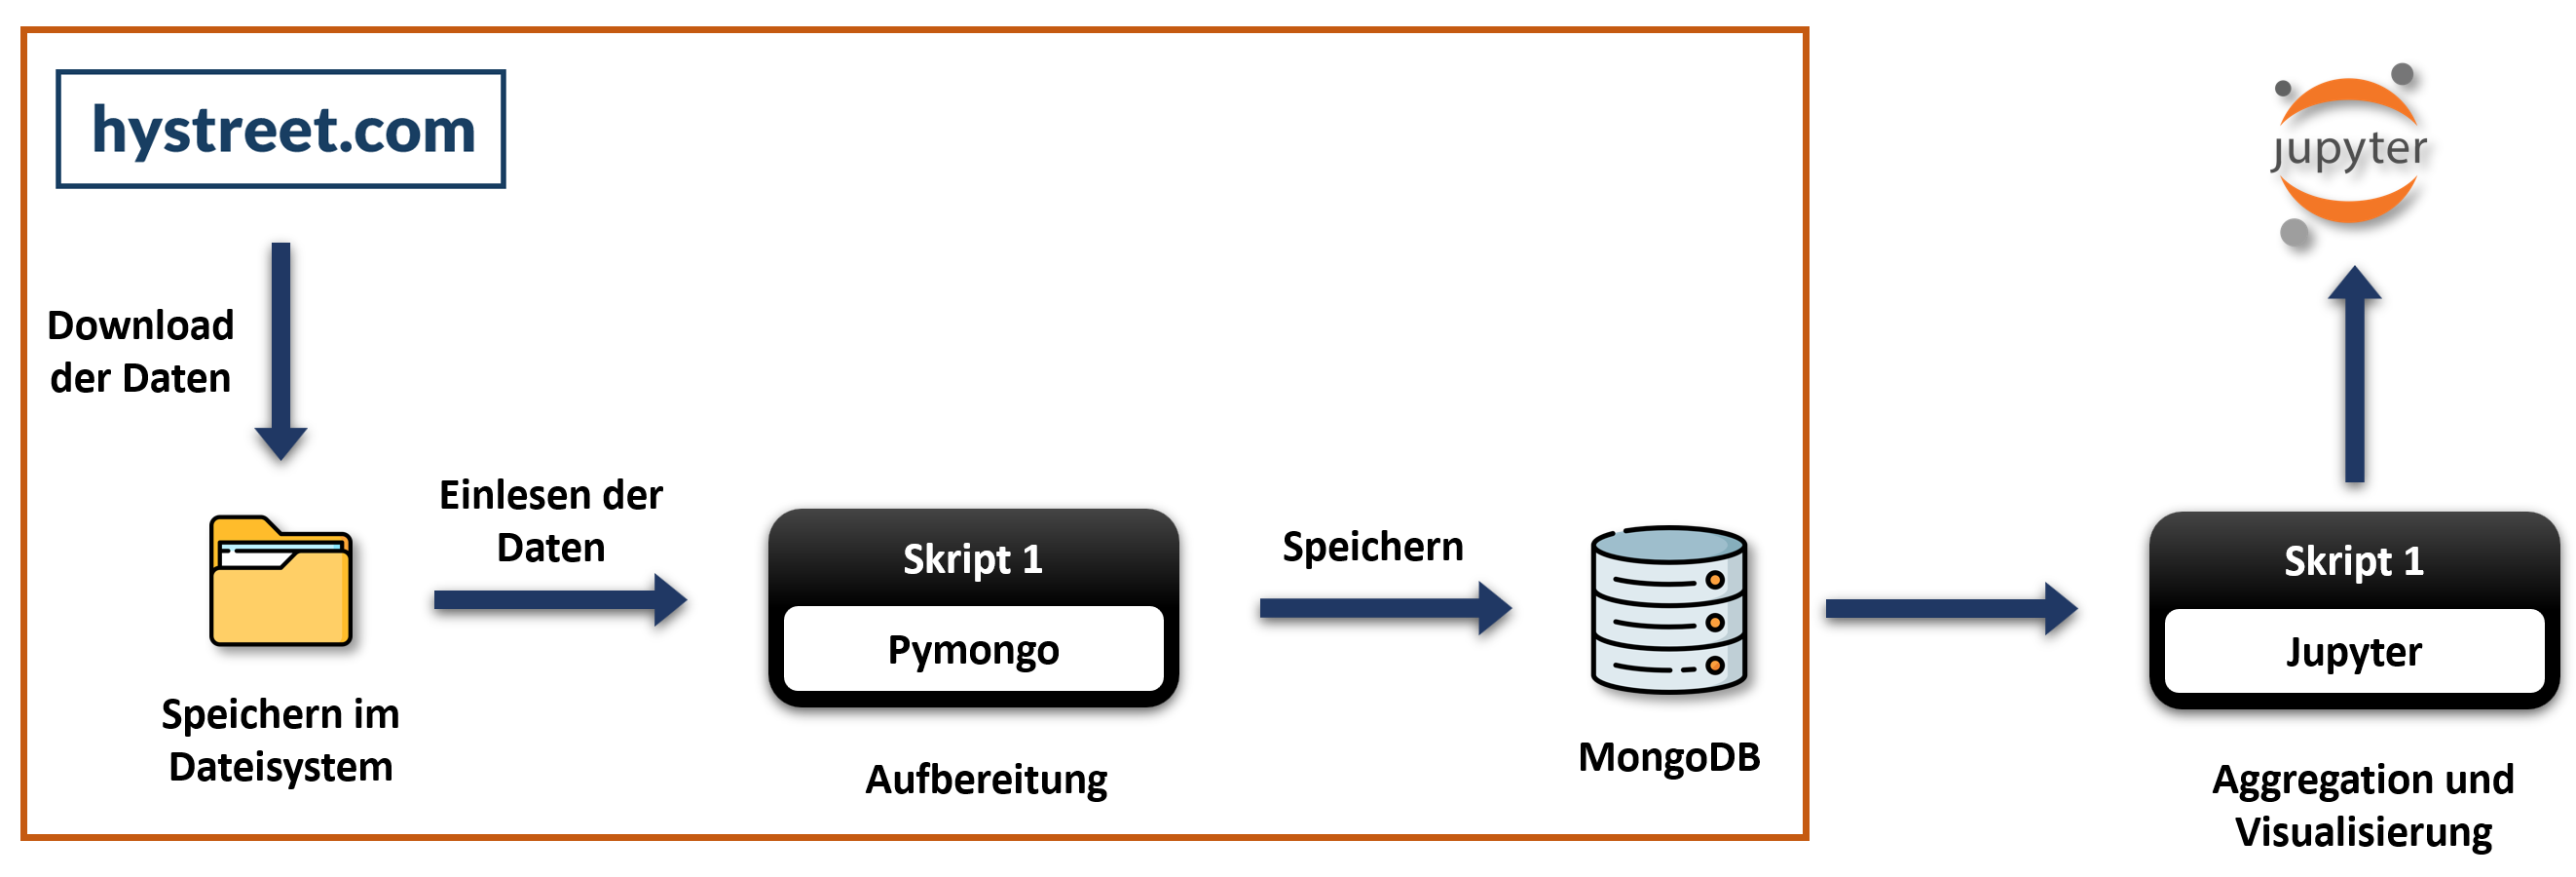
\includegraphics[width=0.8\linewidth]{images/datenpipelineT1.png}
    \caption{Datenpipeline - Einlesen und verarbeiten der Daten}
    \label{fig:datenpipelineT1}
\end{figure}

\subsection{Herunterladen der Daten}
Wie bereits erwähnt stand für uns nur die kostenfreie Alternative zur Verfügung, die Daten manuell über die Webseite für jeden einzelnen Standort herunterzuladen. In Abbildung \ref{fig:hystreet-download} zu sehen ist beispielhaft die Oberfläche der Webseite zum Herunterladen der Daten des Jungfernstegs in Hamburg. Auswählen ist Granularität der Daten, also, ob man die Angaben pro Stunde oder pro Tag möchte und der Zeitraum der gewünschten Daten ist auszuwählen.

\begin{figure}[h!]
    \vspace{0.4cm}
    \centering
    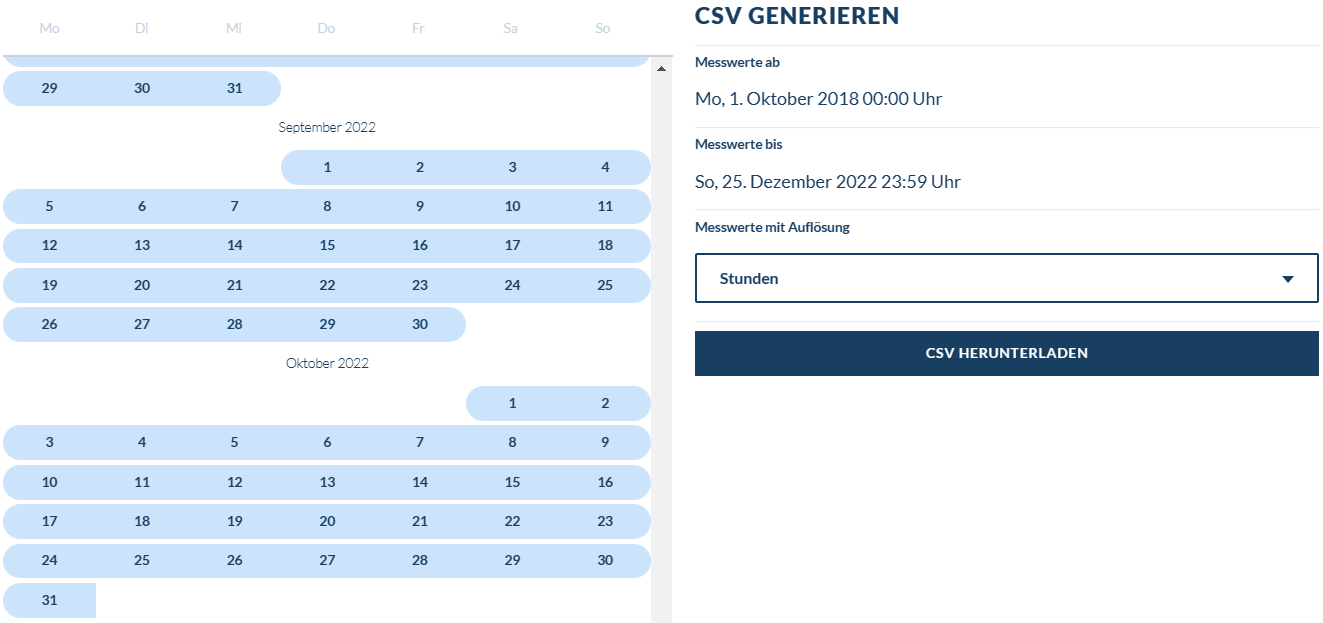
\includegraphics[width=0.9\linewidth]{images/hystreet-datendownload.png}
    \caption{Datenpipeline - Einlesen und verarbeiten der Daten}
    \label{fig:hystreet-download}
    \vspace{0.1cm}
\end{figure}

Dieses Prozedere für jeden gewünschten Standort durchgeführt, erhalten wir die jeweiligen CSV-Dateien. Diese werden im Ordner \emph{input/} gespeichert, der Ordner, aus dem anschließend die Dateien eingelesen werden.

\subsection{Aufbereiten der Daten}
Wir wollen die Daten nun einlesen und anschließend so aufbereiten, dass wir sie später einfacher für die verschiedenen Analysen verwenden können. Das - und auch das Schreiben der Daten in die MongoDB - passiert im \emph{Skript 1}, das ebenfalls in ein Jupyter Notebook integriert ist. Dafür benötigen wir die Packages \emph{pymongo} (für die Verbindung zur MongoDB), \emph{pandas} (zum Arbeiten mit den Daten), \emph{json} (zum konvertieren von Daten in das JSON-Format) und \emph{os} zum interagieren mit dem Dateisystem.
\bigbreak

Nachdem wir die Packages importiert haben und die Datein im Ordner \emph{input/} aufgelistet haben, lesen wir diese jeweils in ein eigenes Pandas-Dataframe ein und speichern sie gemeinsam in einer Liste.

\bigbreak
\begin{tcolorbox}[breakable, size=fbox, boxrule=1pt, pad at break*=1mm,colback=cellbackground, colframe=cellborder]
\prompt{In}{incolor}{1}{\boxspacing}
\begin{Verbatim}[commandchars=\\\{\}]
\PY{n}{files} \PY{o}{=} \PY{p}{[} \PY{l+s+s1}{\PYZsq{}}\PY{l+s+s1}{data/}\PY{l+s+s1}{\PYZsq{}} \PY{o}{+} \PY{n}{x} \PY{k}{for} \PY{n}{x} \PY{o+ow}{in} \PY{n}{os}\PY{o}{.}\PY{n}{listdir}\PY{p}{(}\PY{l+s+s1}{\PYZsq{}}\PY{l+s+s1}{data}\PY{l+s+s1}{\PYZsq{}}\PY{p}{)} \PY{p}{]}
\PY{n}{data} \PY{o}{=} \PY{p}{[} \PY{n}{pd}\PY{o}{.}\PY{n}{read\PYZus{}csv}\PY{p}{(}\PY{n}{x}\PY{p}{,} \PY{n}{delimiter}\PY{o}{=}\PY{l+s+s1}{\PYZsq{}}\PY{l+s+s1}{;}\PY{l+s+s1}{\PYZsq{}}\PY{p}{)} \PY{k}{for} \PY{n}{x} \PY{o+ow}{in} \PY{n}{files} \PY{p}{]} \PY{c+c1}
\end{Verbatim}
\end{tcolorbox}
\bigbreak

Da wir ausschließlich die Daten der Jahre 2020 - 2022 betrachten werden, werd anschließend eine Funktion erstellt, die die Daten auf genau dieses Kriterium filtert und die gefilterten Daten zurückgibt.

\bigbreak
\begin{tcolorbox}[breakable, size=fbox, boxrule=1pt, pad at break*=1mm,colback=cellbackground, colframe=cellborder]
\prompt{In}{incolor}{2}{\boxspacing}
\begin{Verbatim}[commandchars=\\\{\}]
\PY{k}{def} \PY{n+nf}{filterData}\PY{p}{(}\PY{n}{data}\PY{p}{)}\PY{p}{:}
    \PY{l+s+sd}{\PYZsq{}\PYZsq{}\PYZsq{}Delete all rows where the year is not between 2020 and 2022\PYZsq{}\PYZsq{}\PYZsq{}}
    \PY{k}{for} \PY{n}{i} \PY{o+ow}{in} \PY{n+nb}{range}\PY{p}{(}\PY{n+nb}{len}\PY{p}{(}\PY{n}{data}\PY{p}{)}\PY{p}{)}\PY{p}{:}
        \PY{n}{data}\PY{p}{[}\PY{n}{i}\PY{p}{]}\PY{o}{.}\PY{n}{drop}\PY{p}{(}\PY{n}{data}\PY{p}{[}\PY{n}{i}\PY{p}{]}\PY{p}{[}\PY{p}{(}\PY{n}{data}\PY{p}{[}\PY{n}{i}\PY{p}{]}\PY{o}{.}\PY{n}{year} \PY{o}{\PYZlt{}} \PY{l+m+mi}{2020}\PY{p}{)} \PY{o}{|} \PY{p}{(}\PY{n}{data}\PY{p}{[}\PY{n}{i}\PY{p}{]}\PY{o}{.}\PY{n}{year} \PY{o}{\PYZgt{}} \PY{l+m+mi}{2022}\PY{p}{)}\PY{p}{]}\PY{o}{.}\PY{n}{index}\PY{p}{,} \PY{n}{inplace}\PY{o}{=}\PY{k+kc}{True}\PY{p}{)}
    \PY{k}{return} \PY{n}{data}
\end{Verbatim}
\end{tcolorbox}
\bigbreak

Wir definieren anschließend noch weitere Funktionen, um zusammengesetze Felder in den Daten aufzuteilen. Zu Erinnerung, wir startet mit Daten die wie folgt aussehen:
\begin{table}[h!]
\resizebox{\textwidth}{!}{%
\begin{tabular}{|c|c|c|c|c|c|c|}
\hline
location & time of measuremnt & weekday & pedestrians count & temperature in c & weather condition & incidents \\
\hline
\end{tabular}}
\end{table}

Ziel und Ergebnis der aufbereitung der Daten ist folgenden Schema:
\begin{table}[h!]
\resizebox{\textwidth}{!}{%
\begin{tabular}{|c|c|c|c|c|c|c|c|c|c|c|c|}
\hline
address & weekday & pedestrians & temperature & weatherCondition & incidents & location & city & year & month & day & hour \\
\hline
\end{tabular}}
\end{table}

Um dieses Ergebnis zu erreichen, definieren wir noch weitere Funktionen, die die einzelnen dafür benötigten Schritte ausführung und schließlich noch eine Funktion, die prüft, ob alle Daten in allen Städten vollständig sind. Hierbei wird geprüft, ob in allen Städten die gleiche Anzahl an Einträgen vorhanden ist.

Nach der Definition der einzelnen Funktionen, werden diese nur noch auf den ursprünglichen Datensatz angewendet und wir erhalten die aufbereiteten Daten mit dem passenden zuvor beschriebenen Schema.

\bigbreak
\begin{tcolorbox}[breakable, size=fbox, boxrule=1pt, pad at break*=1mm,colback=cellbackground, colframe=cellborder]
\prompt{In}{incolor}{3}{\boxspacing}
\begin{Verbatim}[commandchars=\\\{\}]
\PY{n}{data} \PY{o}{=} \PY{n}{filterData}\PY{p}{(}\PY{n}{data}\PY{p}{)}
\PY{n}{data} \PY{o}{=} \PY{n}{separateLocation}\PY{p}{(}\PY{n}{data}\PY{p}{)}
\PY{n}{data} \PY{o}{=} \PY{n}{separateTime}\PY{p}{(}\PY{n}{data}\PY{p}{)}
\PY{n}{data} \PY{o}{=} \PY{n}{cleanData}\PY{p}{(}\PY{n}{data}\PY{p}{)}
\PY{n}{checkData} \PY{p}{(}\PY{n}{data}\PY{p}{)}
\end{Verbatim}
\end{tcolorbox}
\bigbreak

\subsection{Speichern der Daten}
Der letzte Schritt im \emph{Skript 1} besteht nun nur noch im Einlesen der Daten in die MongoDB. Dafür verwenden wir, wie erwähnt, das Package \emph{pymongo}. Zunächst wird also eine Verbindung zum lokalen MongoDB-Client hergestellt und die Verbindung in einer Variable gespeichert. Anschließend wählen wir über den Client die Database \emph{HyStreet} aus. Bevor wir die Daten nun einlesen, müssen wir diese noch in das JSON-Format überführen, was wir mit der Funktion \emph{DATAFRAME.to\_dict()}, zur Verfügung gestellt von \emph{Pandas}, erreichen. Danach können wir schließlich die Daten in die Collection \emph{HyStreetData} einfügen. 
Damit wir die eingelesenen Dateien beim nächsten Durchlauf des Skripts nicht wiederholt einlesen verschieben wir die Dateien schließlich noch in einen anderen Ordner.

\bigbreak
\begin{tcolorbox}[breakable, size=fbox, boxrule=1pt, pad at break*=1mm,colback=cellbackground, colframe=cellborder]
\prompt{In}{incolor}{4}{\boxspacing}
\begin{Verbatim}[commandchars=\\\{\}]
\PY{n}{client} \PY{o}{=} \PY{n}{pymongo}\PY{o}{.}\PY{n}{MongoClient}\PY{p}{(}\PY{l+s+s1}{\PYZsq{}}\PY{l+s+s1}{mongodb://localhost:27017}\PY{l+s+s1}{\PYZsq{}}\PY{p}{)}
\PY{n}{db} \PY{o}{=} \PY{n}{client}\PY{p}{[}\PY{l+s+s1}{\PYZsq{}}\PY{l+s+s1}{HyStreet}\PY{l+s+s1}{\PYZsq{}}\PY{p}{]}

\PY{k}{for} \PY{n}{i} \PY{o+ow}{in} \PY{n+nb}{range}\PY{p}{(}\PY{n+nb}{len}\PY{p}{(}\PY{n}{data}\PY{p}{)}\PY{p}{)}\PY{p}{:}
    \PY{n}{data}\PY{p}{[}\PY{n}{i}\PY{p}{]} \PY{o}{=} \PY{n}{data}\PY{p}{[}\PY{n}{i}\PY{p}{]}\PY{o}{.}\PY{n}{to\PYZus{}dict}\PY{p}{(}\PY{n}{orient}\PY{o}{=}\PY{l+s+s1}{\PYZsq{}}\PY{l+s+s1}{records}\PY{l+s+s1}{\PYZsq{}}\PY{p}{)}
\PY{k}{for} \PY{n}{i} \PY{o+ow}{in} \PY{n+nb}{range}\PY{p}{(}\PY{n+nb}{len}\PY{p}{(}\PY{n}{data}\PY{p}{)}\PY{p}{)}\PY{p}{:}
    \PY{n}{db}\PY{o}{.}\PY{n}{HyStreetData}\PY{o}{.}\PY{n}{insert\PYZus{}many}\PY{p}{(}\PY{n}{data}\PY{p}{[}\PY{n}{i}\PY{p}{]}\PY{p}{)}

\PY{k}{for} \PY{n}{file} \PY{o+ow}{in} \PY{n}{os}\PY{o}{.}\PY{n}{listdir}\PY{p}{(}\PY{l+s+s1}{\PYZsq{}}\PY{l+s+s1}{data}\PY{l+s+s1}{\PYZsq{}}\PY{p}{)}\PY{p}{:}
    \PY{n}{shutil}\PY{o}{.}\PY{n}{move}\PY{p}{(}\PY{l+s+sa}{f}\PY{l+s+s1}{\PYZsq{}}\PY{l+s+s1}{data/}\PY{l+s+si}{\PYZob{}}\PY{n}{file}\PY{l+s+si}{\PYZcb{}}\PY{l+s+s1}{\PYZsq{}}\PY{p}{,} \PY{l+s+sa}{f}\PY{l+s+s1}{\PYZsq{}}\PY{l+s+s1}{geleseneDateien/eingelesen\PYZus{}}\PY{l+s+si}{\PYZob{}}\PY{n}{file}\PY{l+s+si}{\PYZcb{}}\PY{l+s+s1}{\PYZsq{}}\PY{p}{)}
\end{Verbatim}
\end{tcolorbox}
\bigbreak